% !TeX root = ../main.tex
\chapter{Project Management}

Project management for Jan-Sunwai AI followed an iterative delivery approach with explicit weekly milestones, acceptance checkpoints, and operational hardening gates. The planning strategy balanced feature development with risk reduction, especially in AI reliability, security posture, and deployment reproducibility.



\section{Project Planning}

Project planning translated broad objectives into actionable delivery slices with explicit milestones, quality gates, and integration checkpoints. Planning was intentionally cross-functional, so backend APIs, frontend role flows, AI services, and deployment scripts evolved in synchronized increments rather than in isolated tracks. This structure reduced integration shocks and enabled predictable weekly review cycles.

\subsection{Development Approach and Justification}

The project used an incremental and verification-driven approach with the following cycle:

\begin{enumerate}
\item Build baseline functionality for a module.
\item Validate through unit and integration checks.
\item Expose role workflow in UI and test end-to-end behavior.
\item Add security/performance hardening after functional stabilization.
\item Document operational procedures and release notes.
\end{enumerate}

This approach was chosen over a strict waterfall model because AI behavior and UX patterns required iterative calibration [17, 11, 12].


\subsection{Group Roles and Responsibilities}

The responsibility matrix below defines the cross-functional ownership areas covered during delivery.

\begin{table}[H]
\centering
\small
\caption{Role Responsibility Matrix (Project Execution)}
\begin{tabularx}{\textwidth}{|>{\RaggedRight\arraybackslash}p{0.30\textwidth}|>{\RaggedRight\arraybackslash}X|}
\hline
\textbf{Role Area} & \textbf{Responsibilities} \\ \hline
Backend Engineering & API design, schema validation, business logic, role authorization, lifecycle transitions, notification hooks \\ \hline
Frontend Engineering & Route architecture, role dashboards, analyze/result flow, user session handling, responsive behavior \\ \hline
AI and Classification & Vision model integration, rule engine tuning, reasoning fallback, draft generation quality checks \\ \hline
Data and Persistence & MongoDB collection design, indexes, query access paths, reset token TTL and audit metadata \\ \hline
Security and Reliability & Input sanitization, upload hardening, CORS and headers, degrade behavior, readiness/liveness semantics \\ \hline
Testing and QA & Unit and integration tests, resilience and security validation, load profiling, UAT scripts \\ \hline
DevOps and Deployment & Compose consolidation, environment normalization, production verification scripts, backup runbooks \\ \hline
Documentation and Handover & API reference, deployment guides, user manual, architecture and report compilation \\ \hline
\end{tabularx}
\end{table}

\subsection{Group Dependencies}

The project includes cross-cutting dependencies that were managed explicitly:

\begin{itemize}
\item Backend depends on MongoDB availability and correctly configured environment variables.
\item Analyze flow depends on file storage service and Ollama runtime health.
\item Frontend route behavior depends on cookie-session state and role claims.
\item Assignment quality depends on worker profile completeness (department, approval, service area, status).
\item Production readiness depends on compose health checks, proxy alignment, and secure secret configuration.
\end{itemize}

Dependency risks were controlled through health endpoints, fallback behaviors, and scripted verification routines.

\section{Project Scheduling (Gantt Chart)}

The Gantt chart below provides a visual representation of the project timeline, showing the distribution of foundation, core development, security hardening, and delivery activities across the 18-week execution window.

\begin{figure}[H]
\centering
\IfFileExists{../../images/gantt chart.png}{%
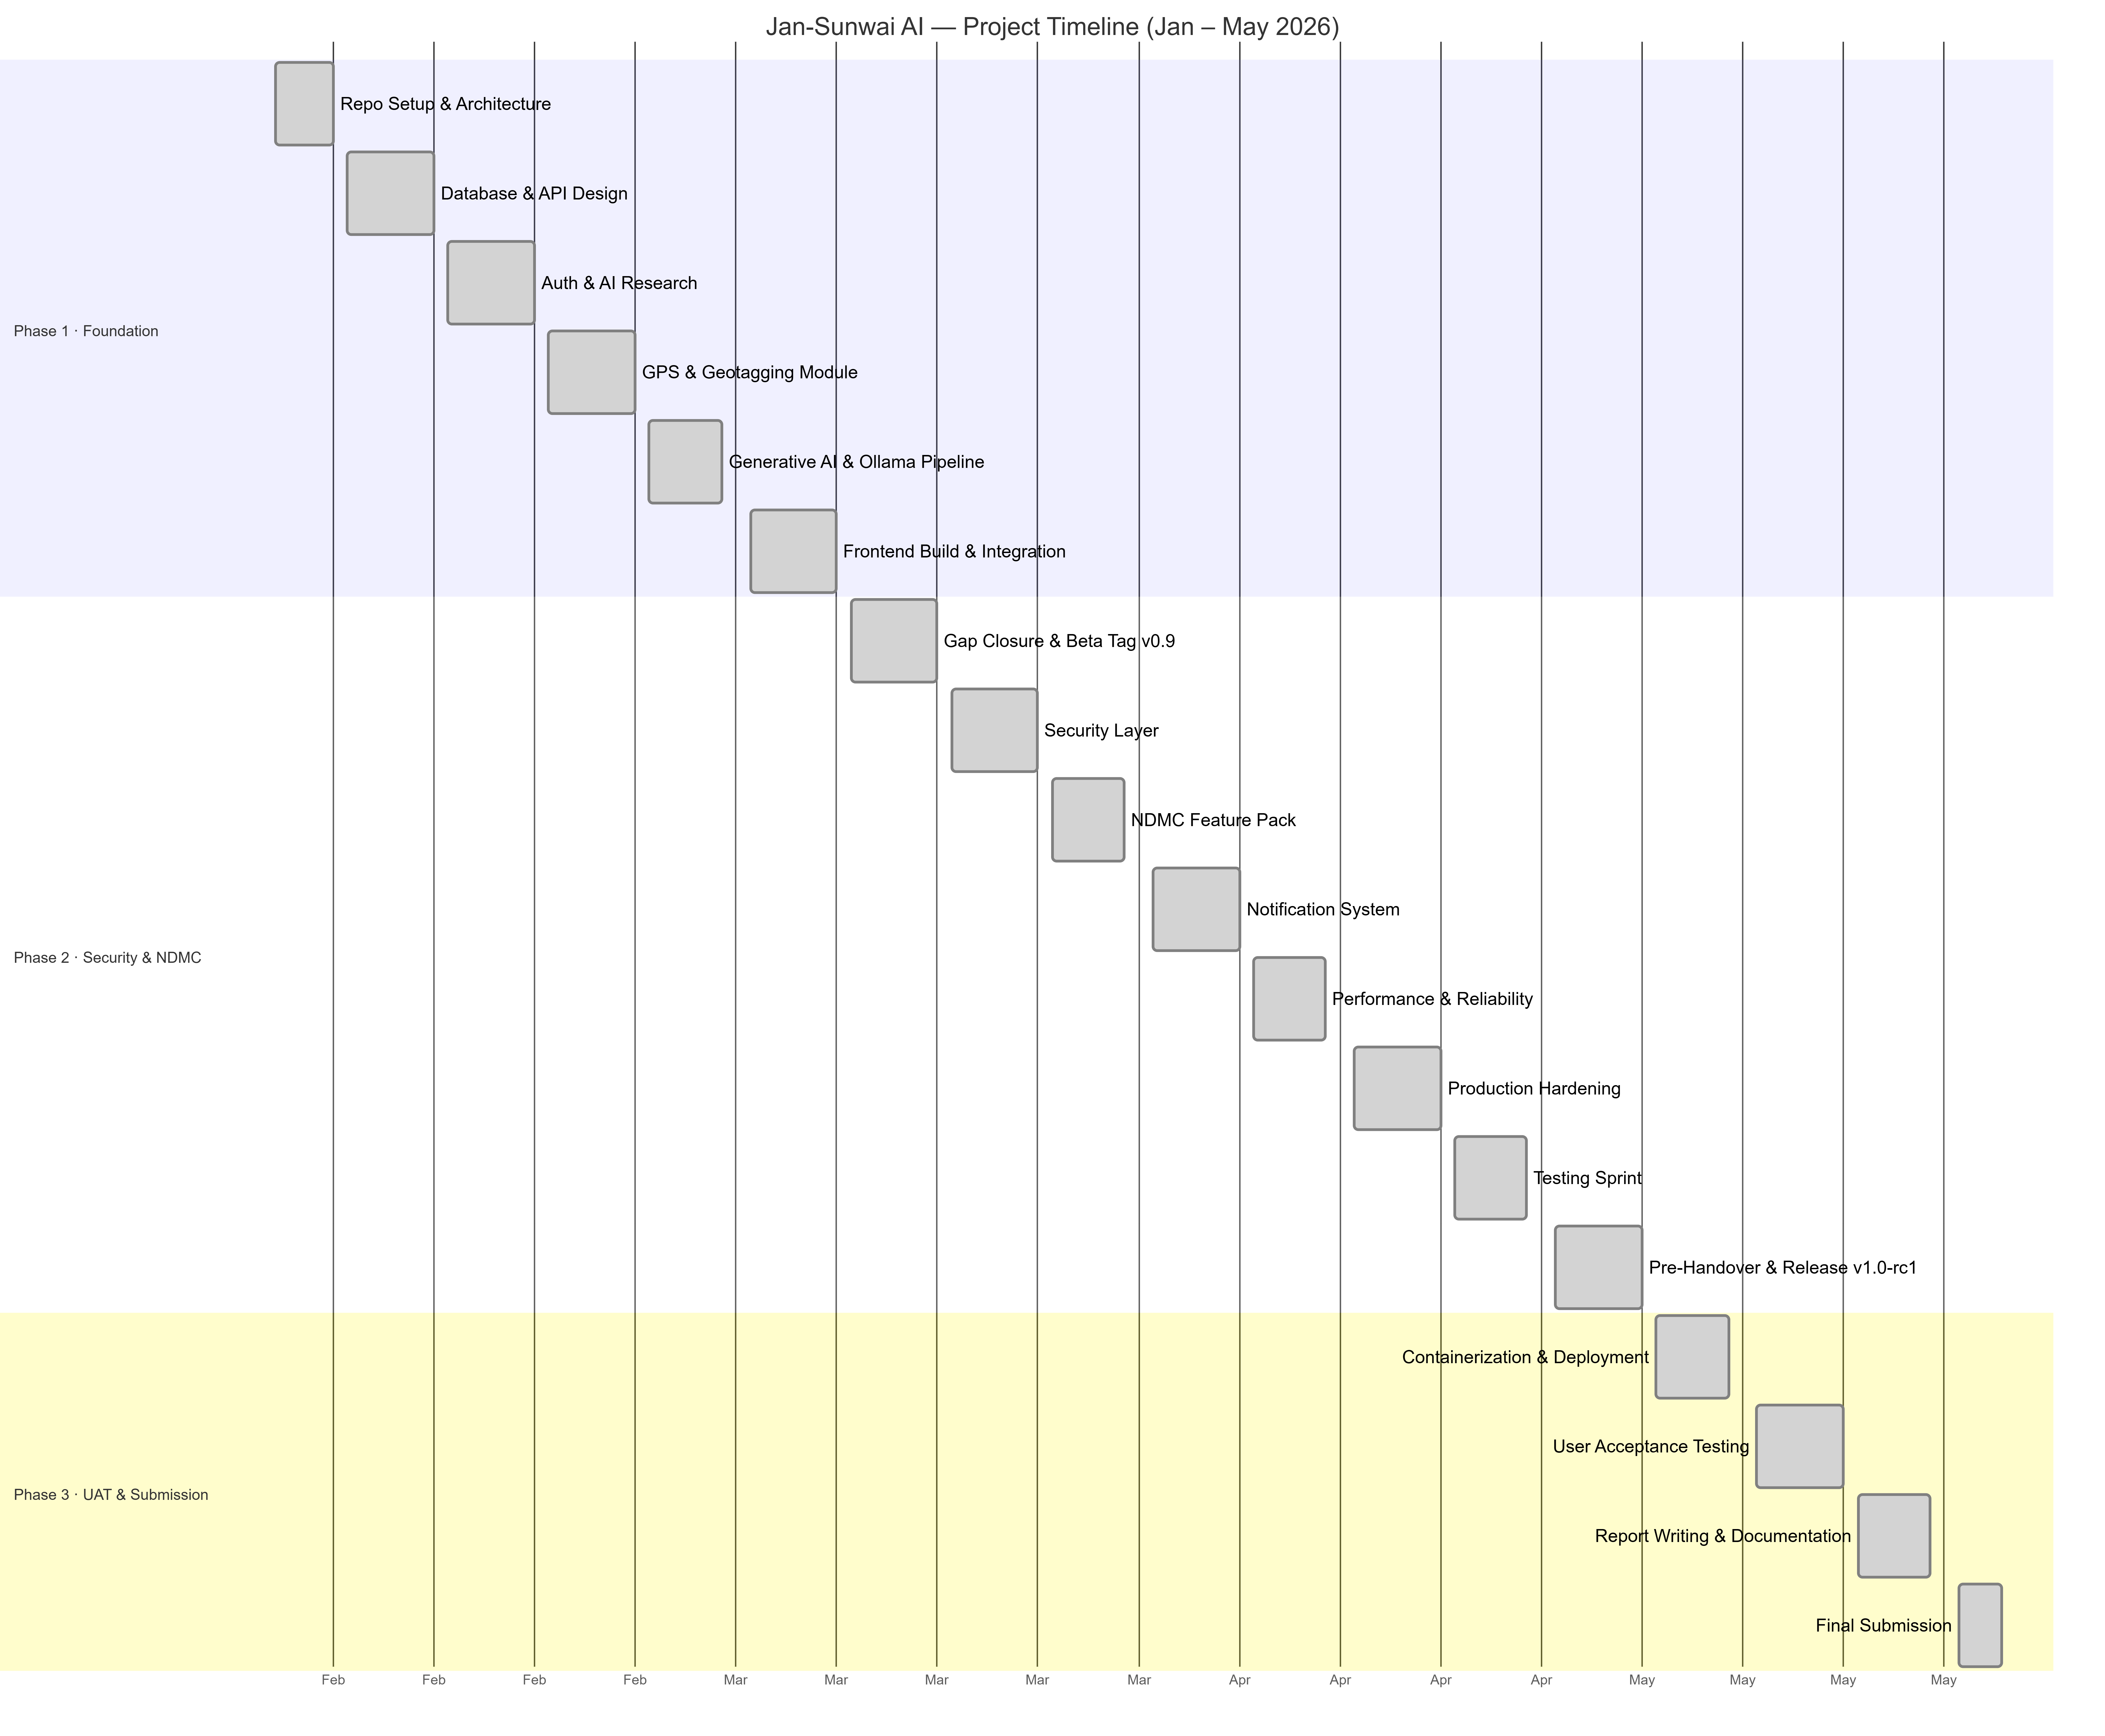
\includegraphics[width=0.95\textwidth]{../../images/gantt chart.png}%
}{%
\fbox{\begin{minipage}[c][0.30\textheight][c]{0.85\textwidth}
\centering Missing Gantt Chart Image
\end{minipage}}%
}
\caption{Jan-Sunwai AI Project Execution Gantt Chart}
\label{fig:gantt-chart}
\end{figure}

\section{Risk Management}

\begin{xltabular}{\textwidth}{|>{\RaggedRight\arraybackslash}X|>{\RaggedRight\arraybackslash}p{0.15\textwidth}|>{\RaggedRight\arraybackslash}p{0.15\textwidth}|>{\RaggedRight\arraybackslash}X|}
\caption{Risk Register and Mitigation Plan}\\
\hline
\textbf{Risk} & \textbf{Likelihood} & \textbf{Impact} & \textbf{Mitigation} \\ \hline
\endhead
Model unavailability or timeout & Medium & High & Multi-tier vision fallback, queue-based generation, retryable 503 responses \\ \hline
Wrong department classification & Medium & High & Deterministic rule engine, triage queue, admin correction workflow \\ \hline
Invalid/malicious uploads & Medium & High & Extension + MIME + magic number + image decode validation, max size enforcement \\ \hline
Unauthorized route access & Low & High & Cookie-session auth (JWT compatibility), role-gated dependencies, integration tests for permission boundaries \\ \hline
Configuration drift across environments & Medium & Medium & Unified backend environment strategy and scripted deployment checks \\ \hline
Notification inconsistency & Low & Medium & Automated notification-chain tests and mark-all-read verification \\ \hline
Performance degradation under load & Medium & Medium & Profiling, timing logs, load-testing matrix, controlled fallback behavior \\ \hline
Documentation mismatch at handover & Medium & Medium & NDMC deployment guide, API reference sync, verification procedure chapter \\ \hline
\end{xltabular}

\section{Management Outcomes}

The management strategy achieved three notable outcomes:

\begin{itemize}
\item Feature breadth was delivered without compromising security and reliability hardening.
\item Delivery confidence increased through continuous testing and issue-driven iteration.
\item Handover readiness improved through consolidated deployment/configuration artifacts and documentation alignment.
\end{itemize}



\section{Chapter Summary}

This chapter demonstrated that the project was not only technically implementable but also deliverable within a controlled timeline and governance framework. Feasibility, dependency management, risk planning, and milestone tracking supported predictable progress toward a production-oriented civic platform.

